\chapter{Logo Retrieval System}\label{c:logoretrievalsystem}

The difficulties of logo retrieval were highlighted in the introduction, in chapter \ref{c:intro}. Nowadays, deep neural networks are utilized to solve such difficult computer vision problems. In this work, end to end neural network solutions will be used, to retrieve logos from videos. The set of logos to be searched is called the query set. Furthermore the frames of videos, where the logos should be retrieved from is called the search set.
\bigbreak
Section \ref{s:logodatasets} details the publicly available logo datasets and introduces a self annotated dataset from sport videos. Section \ref{s:logodetection} shows how Faster R-CNNs can be utilized as logo detectors. Furthermore, section \ref{s:logocomparison} presents the different possibilities how logo image correspondences can be found in a dataset. The chapter is concluded with a solution which includes both tasks in one network.
\bigbreak
\section{Logo Datasets}\label{s:logodatasets}
The hunger of deep learning methods for training data is well-known. This section introduces the datasets, used in this work. First, section \ref{ss:publicdatasets} details the publicly available logo datasets. Since these datasets are relatively small, a better training result can be achieved, if data from the target domain is involved too, and then the datasets are merged. This additional dataset is presented in section \ref{ss:sportlogos}.
\bigbreak
\subsection{Public Datasets}\label{ss:publicdatasets}
The different logo datasets with the number of brands, images and bounding box RoIs can be seen in table \ref{table:logodatasets}. The total number of brands means the number of different brands altogether.

\begin{table}[ht!]
\centering
\begin{tabular}{|l|l|l|l|}
\hline & \textbf{Number of brands} & \textbf{Number of logo images} & \textbf{Number of RoIs} \\
\hline
\textbf{BelgaLogos \cite{belgalogos09}, \cite{letessier2012scalable}} & 37 & 1,321 & 2,697 \\
\hline
\textbf{FlickrBelgaLogos \cite{letessier2012scalable}} & 37 & 2,697 & 2,697 \\
\hline
\textbf{Flickr Logos 27 \cite{619}} & 27 & 810 & 1,261 \\
\hline
\textbf{FlickrLogos-32 \cite{RombergICMR2011}} & 32 & $70 \cdot 32 = 2,240$ & 3,404 \\
\hline
\textbf{Logos-32plus \cite{bianco2017deep}, \cite{bianco2015logo}} & 32 & 7,830 & 12,300 \\
\hline
\textbf{TopLogo10 \cite{DBLP:journals/corr/SuZG16}} & 10 & $10 \cdot 70 = 700$ & 863 \\
\hline\hline
\textbf{Total} & \textbf{80 (union)} & 15,598 & 23,222 \\ \hline
\end{tabular}
\caption{Publicly available logo datasets with bounding box annotations}
\label{table:logodatasets}
\end{table}

There is also a trademark dataset available having a much greater cardinality, called METU Trademark \cite{DBLP:journals/corr/TursunAK17}. However, the images of this dataset contain only the logo of a company, without any context. This dataset turned out to have no use for region-based deep learning methods, since this approach needs to learn to distinguish between objects and the background. The network was trained with the fusion of FlickrLogos-32 and METU trademark dataset. The training setup is described in section \ref{ss:solution5}. Afterwards, it was tested with the evaluation method of py-faster-R-CNN \cite{Girshick2017} \cite{NIPS2015_5638}, described in chapter \ref{c:experiments}.
\bigbreak
However, this training data is insufficient to train a network from scratch (with randomly initialized weights). Girshick et. al. showed \cite{DBLP:journals/corr/GirshickDDM13}, that initializing the weights of the network from a CNN, which was trained on an unrelated dataset, and fine-tuning on the target dataset, can boost on performance significantly. It is because of the hierarchical learning of shapes by the layers of the convolutional neural network. As a result, the learning of the first several convolutional layers can even be turned off during fine-tuning. Thus, for all the training in this work, the weights of models are initialized from a network, pretrained on ImageNet classification dataset \cite{imagenet_cvpr09}.
\bigbreak
\subsection{Self Annotated Dataset - SportLogos}\label{ss:sportlogos}
For dataset extension and evaluation purposes, there were four additional datasets created by extracting them from sport videos. These data are needed, to be able to fine-tune the networks for the specific context. All the logos of these images were annotated despite occlusion and bad sight of them, along with company name. The collected datasets are summarized on table \ref{table:ownlogodatasets}. The utilization of the datasets (training or evaluation) are indicated too. The one, used for testing, is from a different TV broadcasting company than the other three sets, and contains logos which are very challenging to retrieve.
\bigbreak
\begin{table}[ht!]
\centering
\begin{tabular}{|l|l|l|l|l|}
\hline & \textbf{Phase} & \textbf{Number of brands} & \textbf{Number of logo images} & \textbf{Number of RoIs} \\
\hline
\multicolumn{1}{|l|}{\textbf{Football-1}} & \multirow{3}{*}{Train} & \multicolumn{1}{l|}{104} & \multicolumn{1}{l|}{331} & \multicolumn{1}{l|}{3,329} \\\cline{1-1}\cline{3-5}
\multicolumn{1}{|l|}{\textbf{Ski}} & & \multicolumn{1}{l|}{27} & \multicolumn{1}{l|}{179} & \multicolumn{1}{l|}{701} \\\cline{1-1}\cline{3-5}
\multicolumn{1}{|l|}{\textbf{Ice hockey}} & & \multicolumn{1}{l|}{19} & \multicolumn{1}{l|}{410} & \multicolumn{1}{l|}{3,920} \\\hline
\textbf{Football-2} & Test & 40 & 298 & 2,348 \\ \hline
\end{tabular}
\caption{Collected logo datasets from sport videos}
\label{table:ownlogodatasets}
\end{table}
\bigbreak
\subsection{Dataset Fusion}\label{ss:datasetfusion}
Figure \ref{f:branddistribution} summarizes the distribution of the number of logo brands in the fusion of the public and the SportLogos dataset. The latter introduces a large number of classes with low number of examples. Although, these classes are valuable for the training of a logo detector, their usefulness to train a classifier is doubtful.
\begin{figure}
  \centering
  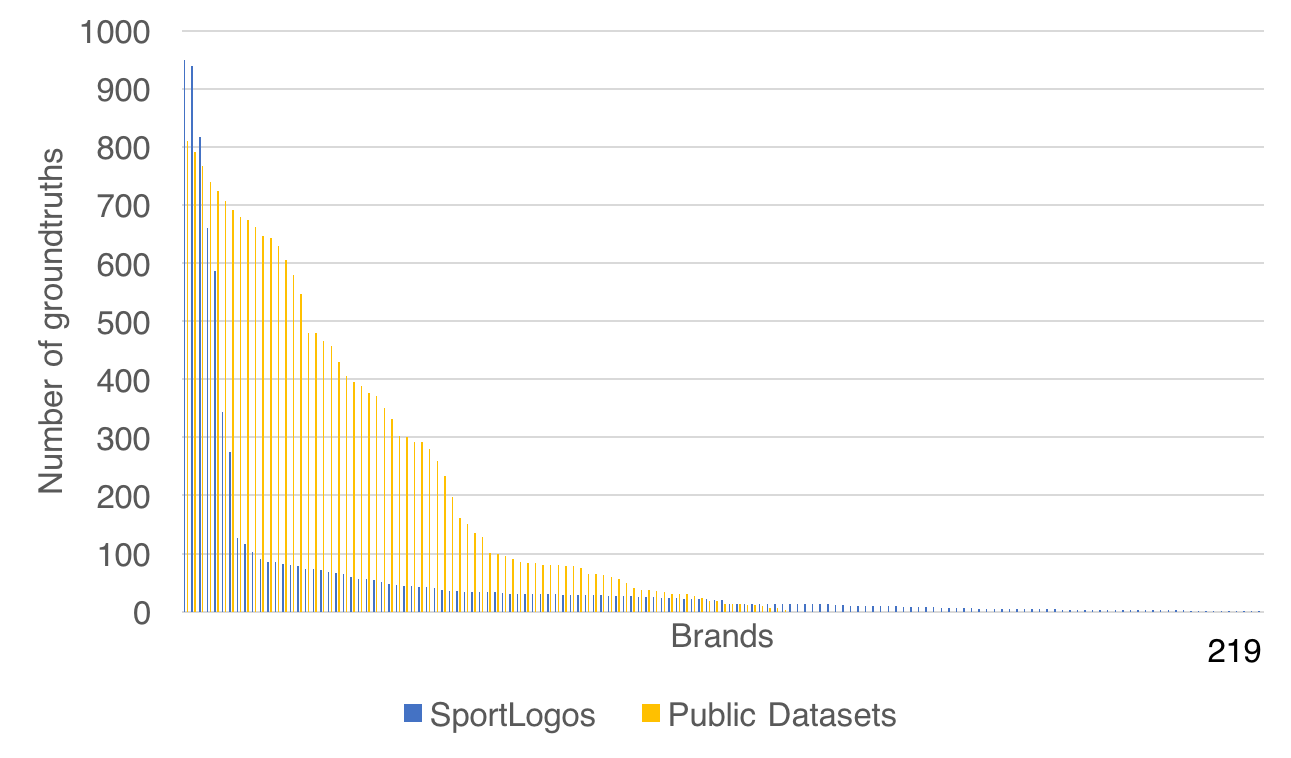
\includegraphics[width=100mm]{images/mt/branddistribution.png}
  \caption{Cardinality of different brands in the public and SportLogos datasets}
  \label{f:branddistribution}
\end{figure}
The SportLogos dataset contains some brands, which are already in the set of public datasets. After fusing the datasets with the logos of 218 brands, it already includes the logos of a lot of common sport brands. Thus, it is hard to find a sport video with logos, which cannot be already found in the training set. The figure \ref{f:commonbrands} presents the extent of intersections. This means, that four brands are already comprised by the training data, from which two are negligible, because of having fewer than five training examples. The effect of other two classes will be examined further in chapter \ref{c:experiments}. The list of all brands and the number of contained ground-truths can be found in the Appendix.
\begin{figure}
  \centering
\begin{tabular}{cc}
  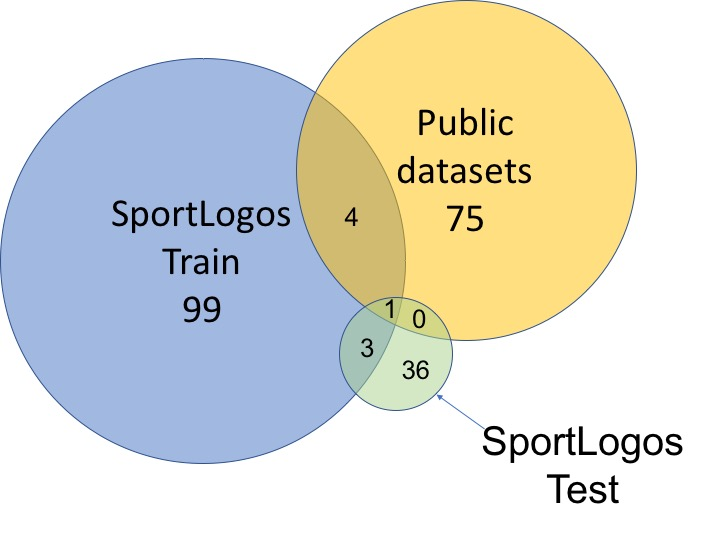
\includegraphics[height=40mm]{images/mt/brandintersections.jpg} &   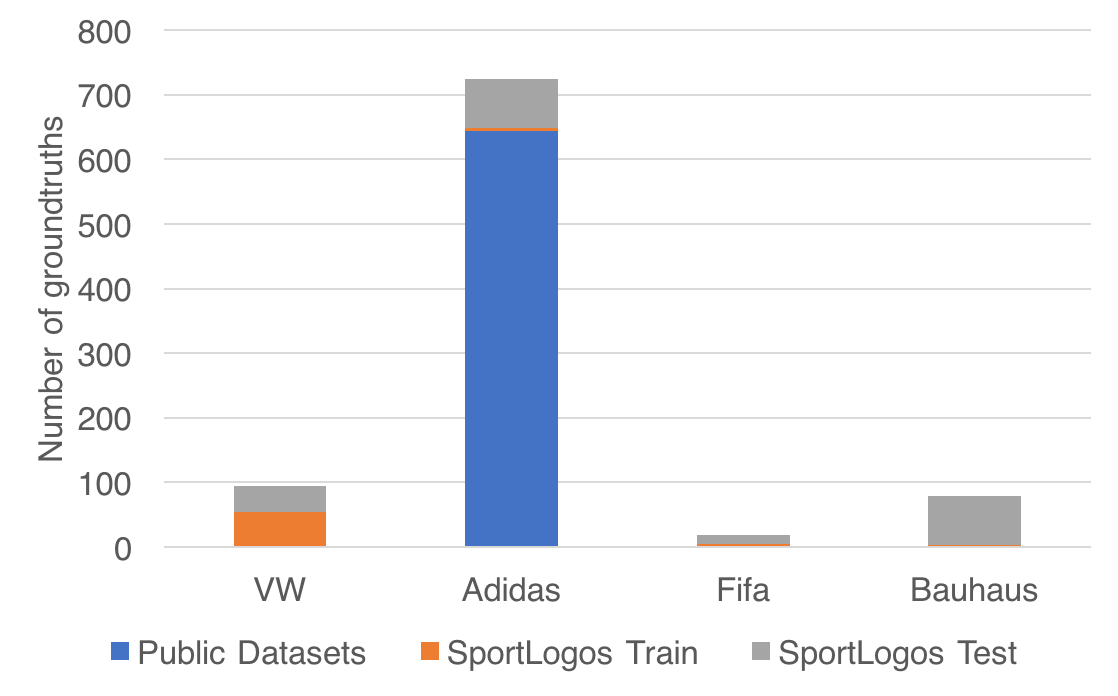
\includegraphics[height=60mm]{images/mt/commonbrands.png}
\end{tabular}
\caption{Left: Number of classes within the different datasets, and their size of intersections. Right: Brands contained by both the training and the test dataset and their cardinality}
\label{f:commonbrands}
\end{figure}
\section{Logo Detection}\label{s:logodetection}
For scene retrieval it is conventional, that one feature is created for an input image. This is achieved either by inferring from the complete image or by searching for key regions and then extracting features from the found regions, which are then finally fused into a global feature. For logo retrieval the goal is not the extraction of a global feature, because it would not be descriptive enough to retrieve small objects. Additionally, a global feature usually does not preserve information of the location and the size of the objects, which are also important factors for logo retrieval.
\bigbreak
Therefore, first the objects should be detected in the input image. There are a lot of possibilities to search for objects as explained in chapter \ref{c:relatedwork}. Keypoint detectors and external proposal systems are translation and rotation invariant, but usually these systems cannot be trained on a specific dataset. Girshick et.al. \cite{NIPS2015_5638} proposed the Faster R-CNN, detailed in section \ref{s:fasterrcnn}, for end to end learning to detect and classify objects on an image. This network has a bounding box regressor for each trained class, thus it is capable to produce object type specific region proposals.
\bigbreak
In the following sections, different detectors will be introduced.
\bigbreak
\subsection{Region Proposal Network}
During the training of a Faster R-CNN, a Region Proposal Network will be trained to detect all kind of objects, which it was trained on. Thus, after training a Faster R-CNN with different logos, the trained RPN can be used alone as a logo detector. It has the advantage, that the detector can be extracted from every already trained Faster R-CNN, unlike those in case of the following solutions.
\bigbreak
\subsection{Class Agnostic Faster R-CNN}\label{ss:classagnosticdetector}
Faster R-CNN can be trained for two classes: background and logo. For this purpose the classes of every annotation box will be neglected. This solution is expected to yield better performance than the RPN detector. Firstly, because of the fully connected layers preceding the final classifier and the bounding box regression layers. Secondly, it is a cascade of two detectors (RPN and FC), similarly as in \cite{Viola:2004:RRF:966432.966458}, where the RPN is a weaker classifier, which is faster, allowing more false positives. For the combination it is expected to have a lower false positive rate.
\begin{figure}
  \centering
  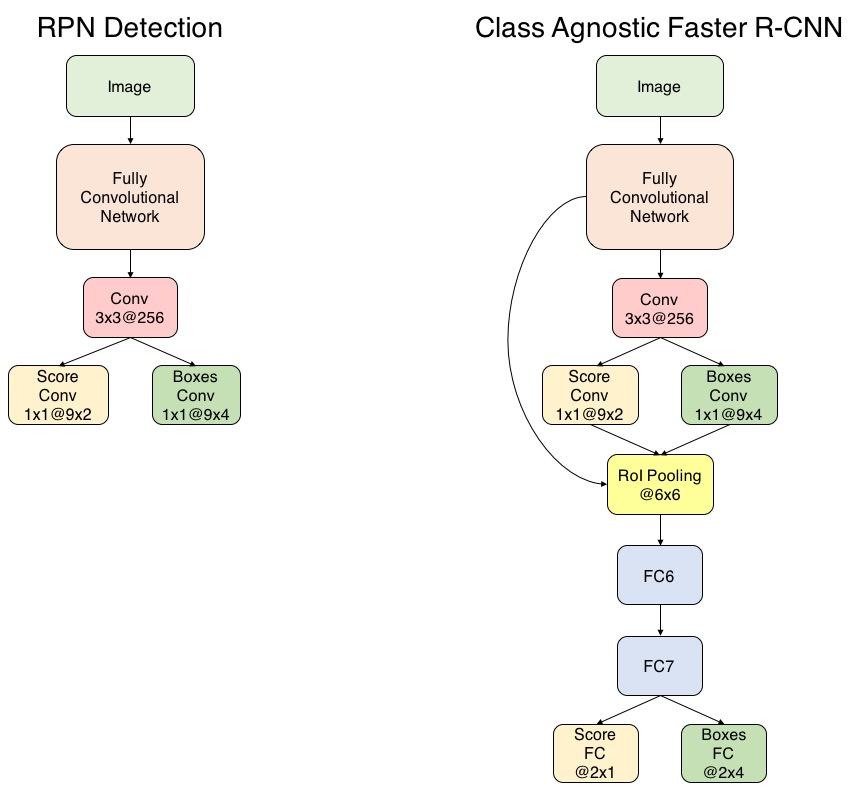
\includegraphics[width=100mm]{images/mt/detectors.jpg}
  \caption{Left: Object detection with Region Proposal Network. Right: Object detection with Faster R-CNN. It can be considered as cascade of a weak and a stronger classifier}
  \label{f:detectors}
\end{figure}
\section{Logo Comparison}\label{s:logocomparison}
After a logo is detected, a correspondence from the query set should be found. In order to retrieve as much objects from the images as possible, the detectors should work with a high recall. Although, for difficult tasks like open-set logo detection, high recall values induce low precision, thus a lot of false positive possible object locations are produced. These examples should be eliminated by the classifier.
\bigbreak
However, in case of image retrieval the goal is not direct classification, but rather feature extraction of an RoI. Thus, the features of the logos of all the query images and the search set should be collected, which can be solved in several ways, detailed in this sections. The retrieved feature vectors are then normalized and the similarities of them are calculated either with euclidean distance or cosine similarity. The similarity score of the former is computed by calculating the L2 (euclidean) norm of difference of the two vectors, then it is placed in the following formula:
\begin{equation}
        \frac{1}{1 + L2(f_1 - f_2)}
        \label{eq:iou}
\end{equation}
whereas $f1, f2$ are the two features to be compared. The cosine distance is computed by calculating the cosine value of the angle between two vectors. For normalized features the magnitude information of the vector is discarded thus, the two distance metrics yield the same results. The distance is then used as probability score of the correspondence to a query image. The detections on a particular location, not having the largest score, are eliminated by non-maximum suppression, which searches for other bounding boxes with a minimum IoU of 0.3.
\bigbreak
\subsection{Baseline: Faster-Logos}\label{ss:solution1}
The features of both the query and the search set can be extracted by running a Faster R-CNN on them in a standard way, and utilizing the output vectors of the last or the second last layer as features. The advantage of this solution is its speed. This is the fastest solution among the detailed ones. But there are several drawbacks. It has low performance, because of the unknown classes, especially if the net is trained for a small number of classes. This results in a low dimensional feature vector e.g. 32 after training with FlickrLogos-32 by using the class probabilities as feature which yields often the best descriptor.
\bigbreak
The Region Proposal Network outputs several hundred possible object locations (default is 300 in test phase) for every input image. Processing so many query features would immensely increase the computational burden. Thus, it is advantageous to filter the detection list. Although, this cannot be done with the classification scores, because the images contain logos from unknown brands, so the descriptors are rather a collection of different brands. For this purpose, the score output of the RPN can be used, which is an objectness indicator. This score can be adopted for the detections of the search images too. Therefore, one can take the RoI with the greatest score for query images, and set a low threshold for images of the search set. The proposed regions are then adjusted with the bounding box regression of the class with the highest probability score. Figure \ref{f:sol1arch} shows the outline of this solution. This solution is chosen for baseline, because it is prevalent in recent research of closed-set logo retrieval in \cite{Bao:2016:RCL:3007669.3007728}, \cite{DBLP:journals/corr/OliveiraFPR16}, \cite{DBLP:journals/spl/QiSWX17}.
\begin{figure}
  \centering
  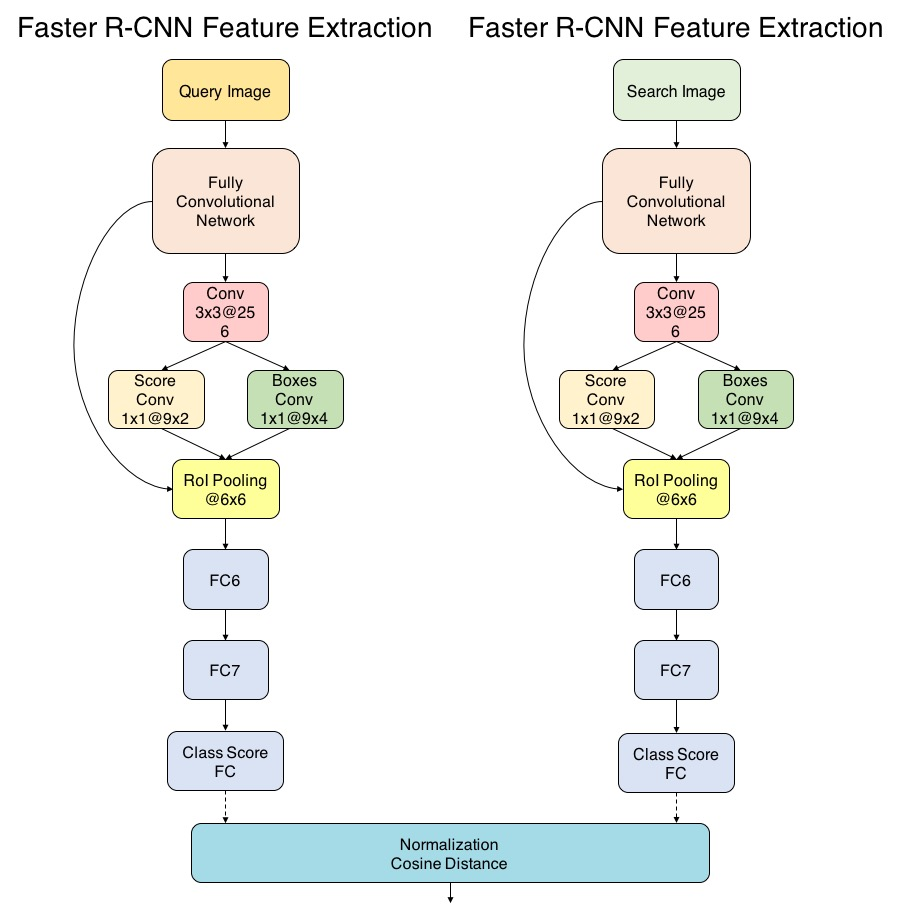
\includegraphics[width=90mm]{images/mt/sol1_arch.jpg}
  \caption{Baseline logo retrieval system applies Faster-R-CNN both on the images of the query and the search set, then compares the features}
  \label{f:sol1arch}
\end{figure}
A next issue, which discourages from applying this method for open-set retrieval, occurs during running the network on the query examples. The network often does not estimate the complete logo with the greatest score, but only a part of that (see the Registered Trade Mark symbol in figure \ref{f:missdet}). This mislocalization destroys the retrieval of that entire class.
\begin{figure}
  \centering
  
\includegraphics[width=25mm]{images/mt/missdet.jpg}
  \caption{Misplaced logo detection, with maximum RPN score}
  \label{f:missdet}
\end{figure}
\subsection{Fast\&Faster-Logos}\label{ss:solution2}
The drawbacks of the solution in section \ref{ss:solution1} imply, that the RPN should be turned off for the examples of the query set. This means, that the network is applied in fast R-CNN mode. For external region proposal one region is applied, which includes the complete query image. However, it may yield worse descriptors, because of the loosely fitting bounding box. On the other hand, the logo positions and their features of the search set can be inferred with Faster R-CNN, and filtered with a threshold as described in section \ref{ss:solution1}.
\begin{figure}
  \centering
  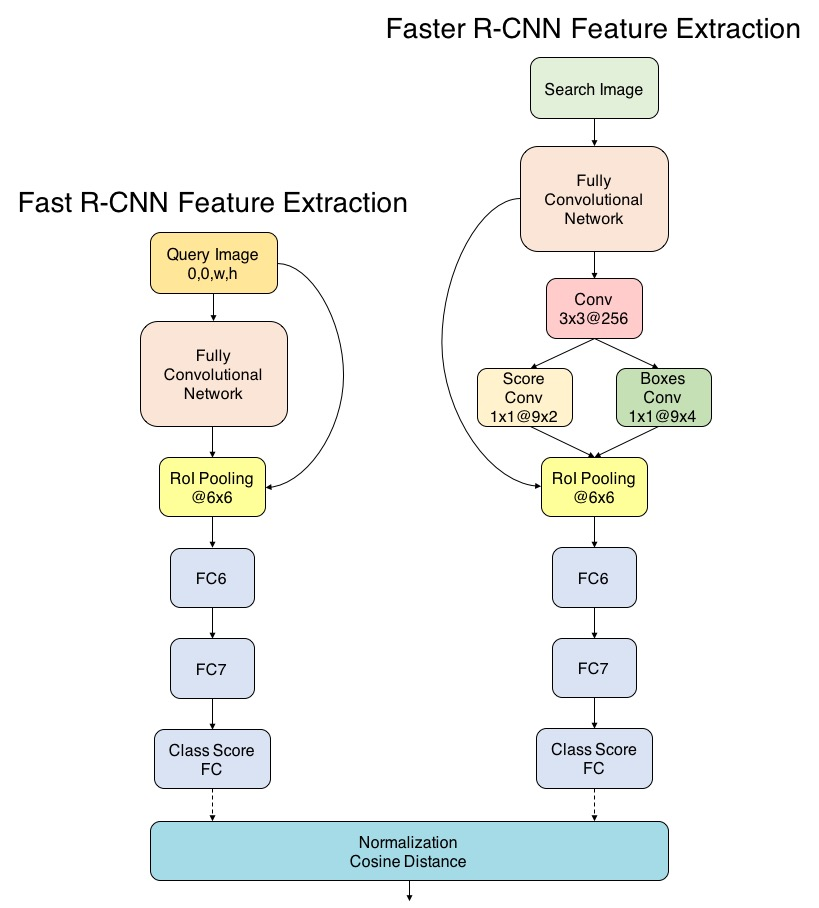
\includegraphics[width=90mm]{images/mt/sol2_arch.jpg}
  \caption{Fast\&Faster-Logos solution. It computes the query feature from the complete query image (i.e. Fast-R-CNN mode), the features of the search image is collected by Faster-R-CNN}
  \label{f:sol2arch}
\end{figure}
\subsection{Fast-Logos}\label{ss:solution3}
The system in section \ref{ss:solution1} may suffer from the inability of the RPN to localize unknown logos. The solution can be further improved by using the best logo detector from the section \ref{s:logodetection}.  The output of the detector is then treated as external proposals, and thus the system runs in fast R-CNN mode for the images of the search set. This setup is very similar to the one of fast R-CNN, detailed in section \ref{s:fastrcnn}, but utilizes neural networks instead of selective search as external region proposal system to collect object locations.
\begin{figure}
  \centering
  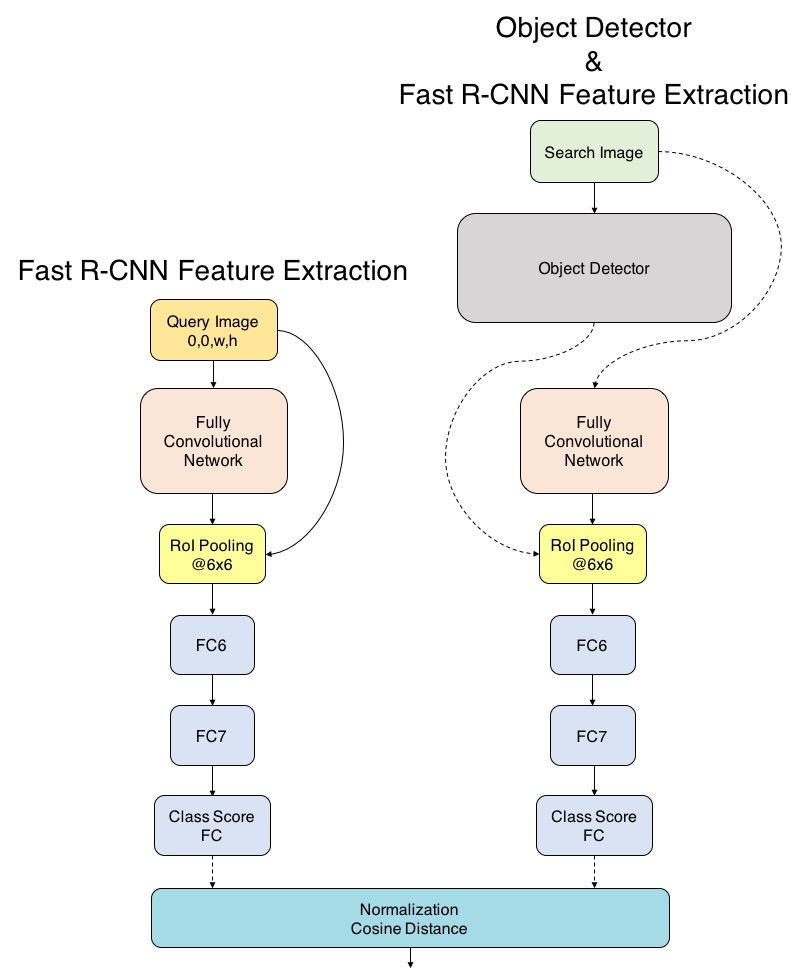
\includegraphics[width=90mm]{images/mt/sol3_arch.jpg}
  \caption{Fast-Logos solution. It computes the features both from the query and the search set in Fast-R-CNN mode, whereas the query region is the complete query image and the locations for the search set come from an external Faster-R-CNN logo detector. The dashed lines indicate and indirect connection between the networks.}
  \label{f:sol3arch}
\end{figure}
\subsection{R-CNN-Logos}\label{ss:solution4}
Section \ref{s:convnets} details the evolution of convolutional networks by going through the most important ones of today. Donahue et al. proposed \cite{DBLP:journals/corr/DonahueJVHZTD13}, that convolutional networks can produce excellent descriptors of the input image, regardless of the absence of fine-tuning to the specific context of the image. For this purpose, a network is pretrained on very large datasets, after which it can be deployed for a broad set of computer vision problems. But it cannot localize objects on an image. For region proposal purpose, a trained logo detector can be utilized from section \ref{s:logodetection}. This setup of networks is very similar to the R-CNN, detailed in section \ref{s:rcnn}, but omits the use of selective search as external region proposal system. As such,it has the disadvantage of retrieving features of the regions separately from each other by not sharing the computed feature maps. Thus, it needs much more time, to infer a complete image. On the other hand, it is beneficial for the performance, because the complete network is only focused on a specific region. This part of the system can be easily swapped to reach the desired performance and time constraints, since all the kind of networks, explained in section \ref{s:convnets} can be utilized for feature extraction. Figure \ref{f:sol4arch} outlines this solution.
\begin{figure}
  \centering
  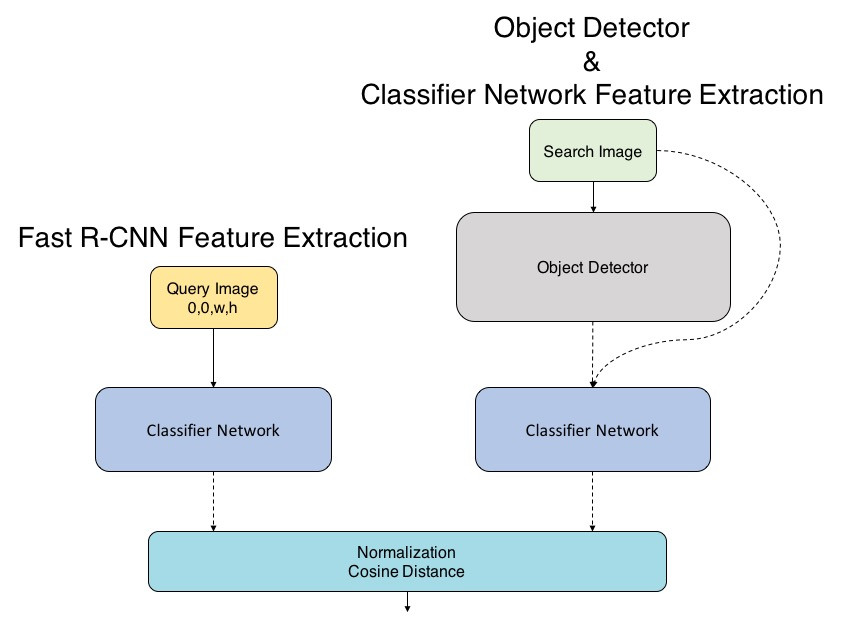
\includegraphics[width=90mm]{images/mt/sol4_arch.jpg}
  \caption{R-CNN-Logos solution. Query region is the complete query image, the search region proposals are generated fromand external Faster-R-CNN logo detector. The features are extracted with a general purpose convolutional network. The dashed lines indicate and indirect connection between the networks.}
  \label{f:sol4arch}
\end{figure}

\subsection{Siam-Logos}\label{ss:solution5}
Both a class agnostic detector (section \ref{ss:classagnosticdetector}) and a classifier can be built together in a Faster R-CNN and trained jointly. For this purpose, either all fully connected layer or only the two at the end of the network, responsible for classification and bounding box regression should be duplicated. In so doing, one branch will be trained with brand label, the other only with logo object indication. In this network, the weights of the feature extraction layers and the Region Proposal Network can be shared between the two tasks. The easiest way to train such a network is a siamese like Faster R-CNN. A schematic illustration of the training and test setup can be seen in figure \ref{f:jointlearning}.
\bigbreak
Siamese networks \cite{Hadsell06dimensionalityreduction} are basically used for calculating similarity scores between inputs. If it is combined with an appropriate loss function e.g. contrastive loss \cite{Hadsell06dimensionalityreduction} or max margin loss \cite{Simonyan13}\cite{ies_2016_herrmann_low_quality}, the network can be trained with an image pair and a label indicating whether the objects on the images are from the same category or not. The network then learns to project objects from the same category with a low-, otherwise with a large distance to each other, according to a specified metric. This is achieved by sharing the weights of the feature extraction layers.
\bigbreak
For Faster R-CNN, the parameters for Region Proposal Network can also be shared. This setup has the advantage, that training of one task can also improve the performance of the other task, which is not currently trained. In particular for logo retrieval, the network can benefit from a bounding box annotated logo dataset, without specific brand indication. To annotate such a dataset much less human resource is needed. A quantitative evaluation can be found in section \ref{s:explogodetection}.
\begin{figure}
  \centering
  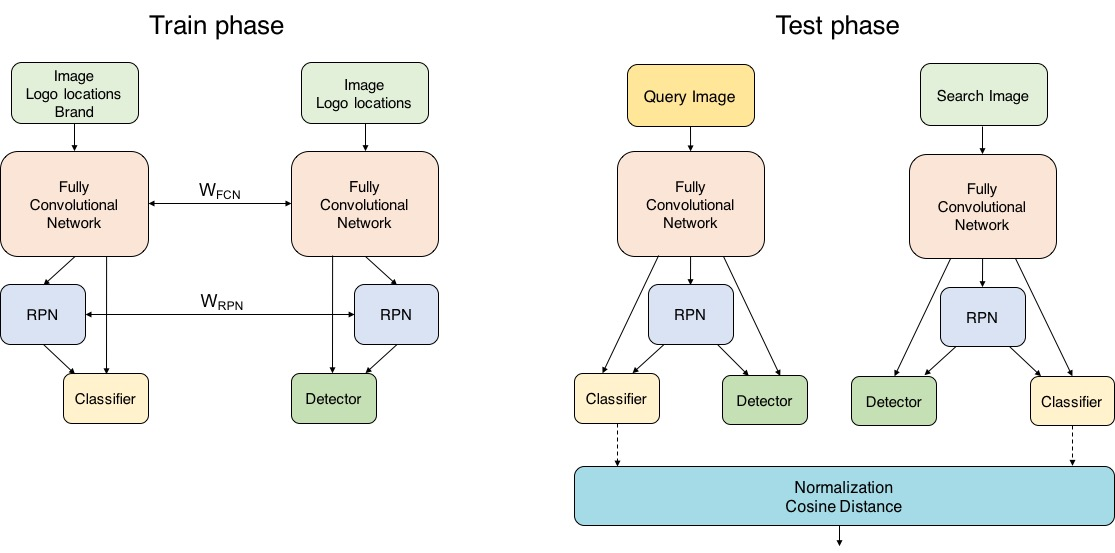
\includegraphics[height=60mm]{images/mt/sol5_arch.jpg}
\caption{Siam-Logos. Network setups in train and test phases for learning detection and classification jointly.}
\label{f:jointlearning}
\end{figure}